\documentclass[../main/main.tex]{subfiles}

\raggedbottom

\makeatletter
\renewcommand{\@chapapp}{\'Electrocin\'etique -- chapitre}
\makeatother

\toggletrue{student}

\begin{document}
\setcounter{chapter}{5}

\chapter{Oscillateurs en r\'egime sinuso\"idal forc\'e}

\section{Introduction}
\subsection{Rappels oscillateurs}

Comme nous l'avions vu au chapitre 4, les oscillateurs amortis caractérisés par
une grandeur physique $x$ sont régis par une équation du type~:
\[ \ddot{x} + \frac{\w_0}{Q} \dot{x} + \w_0{}^2x = \w_0{}^2x_{\eq}\]
Dans le cadre d'un signal d'entrée sinusoïdal $f(t) = A_0\cos(\wt)$ avec une
pulsation $\w$ (i.e. une fréquence $\w/2\pi$), cette équation devient
\[ \ddot{x} + \frac{\w_0}{Q} \dot{x} + \w_0{}^2x = \w_0{}^2f(t) = \w_0{}^2A_0\cos(\wt)\]
avec $A_0$ l'amplitude du forçage. \bigbreak

De la même manière qu'avec une excitation constante ($f(t) = E$ en échelon
montant), la solution de cette équation différentielle sera la somme d'une
solution homogène, caractéristique d'un régime transitoire, et d'une solution
particulière. On a vu que celle-ci prendrait la même forme que le signal
d'entrée, et sera donc également sinusoïdale. On a donc
\begin{gather*}
    x(t) = x_H(t) + x_P(t)\\
    \boxed{x_H(t) \xrightarrow[t\rightarrow+\infty]{} 0}
    \qet
    \boxed{x_P(t) = X\cos(\wt+\f)}
\end{gather*}

On rappelle que le régime sinusoïdal forcé correspond au régime où la solution
homogène est négligeable devant la solution particulière. On aura donc des
solutions de la forme suivante
\begin{center}
    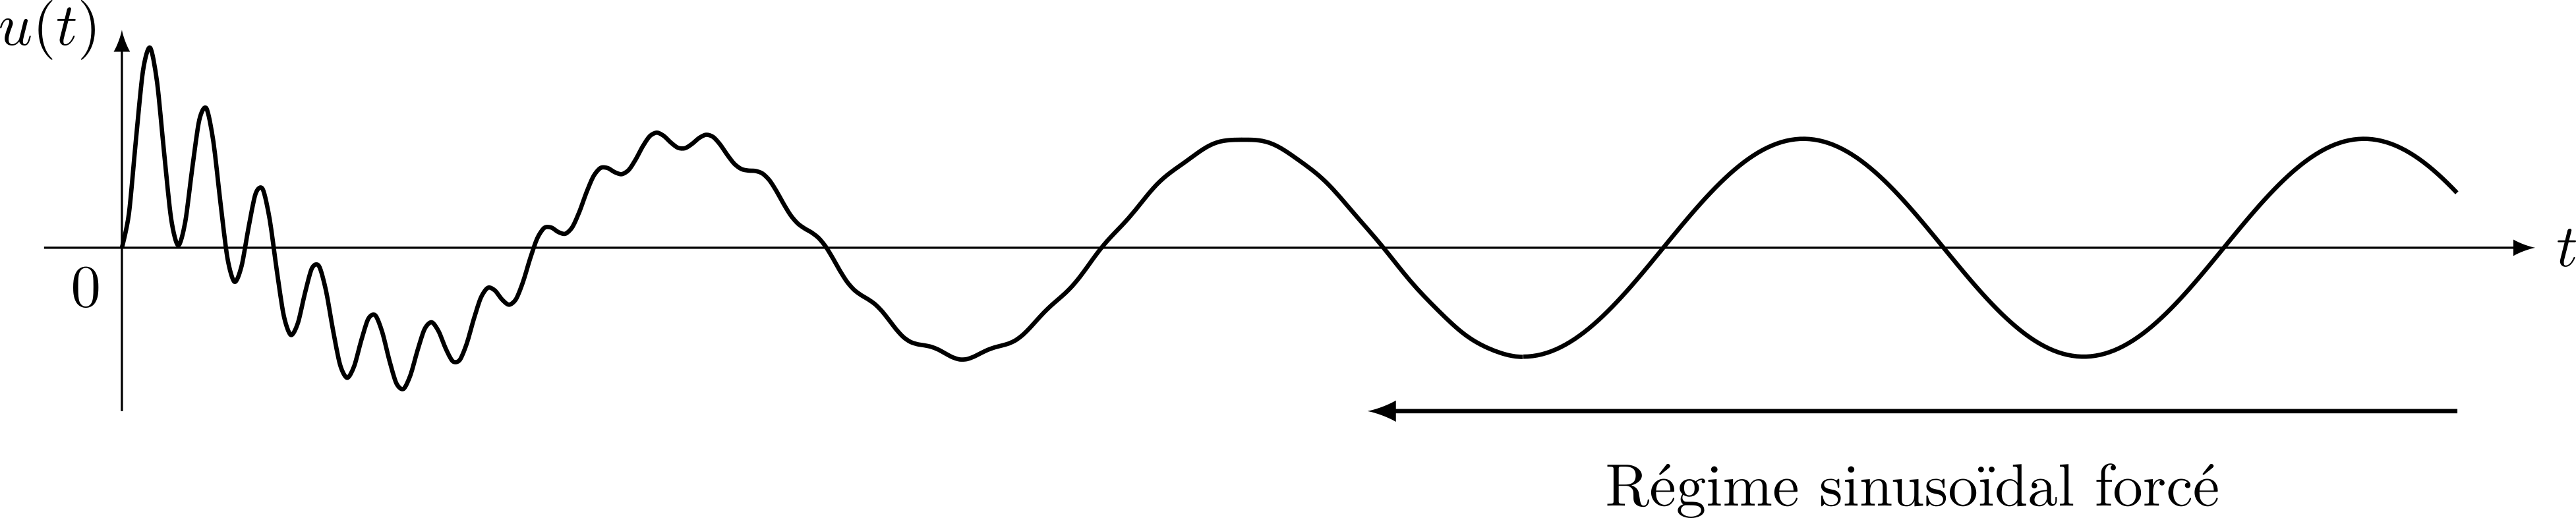
\includegraphics[width=\linewidth]{rsf_intro}
\end{center}
et le but de l'étude de ces systèmes en RSF est de trouver l'amplitude $X$ et la
phase $\f$.

\vspace{-10pt}
\subsection{Méthode des complexes}
Comme dans le chapitre précédent, le passage aux complexes permet d'exprimer
simplement les valeurs de $X$ et de $\f$. Pour passer en complexes, on note
\begin{gather*}
    \boxed{\ul{f}(t) = A_0\exr^{\jj\wt}}
    \qet
    \ul{x}(t) = X\exr^{\jj(\wt+\f)}
    \Leftrightarrow
    \boxed{\ul{x}(t) = \ul{X}\exr^{\jj\wt}}
    \qavec
    \boxed{\ul{X} = X\exr^{\jj\f}}
\end{gather*}
Ainsi, dériver en complexes revient à \textbf{multiplier par $\jj\w$}~: à partir
de l'équation différentielle d'un oscillateur, on aura alors, selon les
exemples, une amplitude de la forme
\[\boxed{
        \ul{X}
        = \frac{A_0}{1 + \jj Q \left( \frac{\w}{\w_r} - \frac{\w_r}{\w} \right)}
}\]

\begin{rror}{Attention}
    Cette forme de résonance n'est qu'un \textbf{exemple}. Elle dépend du
    système.
\end{rror}

% \begin{gather*}
%     \ddot{x} + \frac{\w_0}{Q} \dot{x} + \w_0{}^2x = \w_0{}^2f(t)
%     \Leftrightarrow
%     \ddot{\ul{x}} + \frac{\w_0}{Q} \dot{\ul{x}} + \w_0{}^2\ul{x} = \w_0{}^2\ul{f}(t)\\
%     \Leftrightarrow
%     (\jj\w)^2\ul{x} + \frac{\w_0}{Q}\jj\w\ul{x} + \w_0{}^2\ul{x} = \w_0{}^2\ul{f}(t)
%     \Leftrightarrow
%     \left( \w_0{}^2-\w^2 + \jj \frac{\w\w_0}{Q} \right)
%         \ul{X}\cancel{\exr^{\jj\wt}} = \w_0{}^2A_0\cancel{\exr^{\jj\wt}}\\
%     \Leftrightarrow
%     \ul{X} = \frac{\w_0{}^2A_0}{ \w_0{}^2-\w^2 + \jj \frac{\w\w_0}{Q} }
%     \Leftrightarrow
%     \ul{X} = \frac{A_0}
%         {1 - \left(\dfrac{\w}{\w_0}\right)^2 + \jj \frac{\w}{Q\w_0}}
% \end{gather*}
On trouve donc l'amplitude du signal en en prenant le module~:
% \begin{gather*}
%     X
%         = \left| \ul{X} \right|
%         = \frac{A_0}{
%             \sqrt{\left( 1 - \left(\dfrac{\w}{\w_0}\right)^2 \right)^2
%                 + \left(\dfrac{\w}{Q\w_0}\right)^2}}
% \end{gather*}

\[\boxed{
        X
        = \left| \ul{X} \right|
        = \frac{A_0}{\sqrt{1 + Q^2\left( \frac{\w}{\w_r} - \frac{\w_r}{\w}
        \right)^2}}
}\]

\subsection{Notion de résonance et bande passante}
Par l'étude de l'amplitude, on retrouve bien que $X$ ne dépend pas des
conditions initiales, mais bien de l'amplitude d'entrée mais surtout
\textbf{dépend de la pulsation}. Notamment, on trouve que
\begin{gather*}
    \boxed{X \xrightarrow[\w\rightarrow+\infty]{} 0}
    \qet
    \boxed{X \xrightarrow[\w\rightarrow0]{} 0}
\end{gather*}

Ainsi, il y a une valeur particulière de pulsation telle que l'amplitude est
maximale~: c'est ce qu'on appelle la résonance.

\begin{NCdefi}[width=\linewidth]{Résonance}
    \begin{center}
        \bfseries
        Un oscillateur forcé présente une résonance si l’amplitude de ses
        oscillations est maximale pour une fréquence de forçage finie et non
        nulle. La fréquence correspondante est appelée fréquence de résonance.
    \end{center}
\end{NCdefi}

\begin{minipage}{0.55\linewidth}
    La représentation de l'amplitude en fonction de la pulsation est donc piquée
    autour de son maximum $X_{\max}$ à la pulsation de résonance $\w_r$. Ce pic
    peut être plus ou moins fin, ce que l'on caractérise par la \textbf{bande
    passante}~: c'est le domaine de pulsations du forçage pour lequel $X(\w) >
    X_{\max}/\sqrt{2}$. On définit alors~:
    \begin{itemize}
        \item $\w_1$ et $\w_2$ les \textbf{pulsations de coupure}~;
        \item $\D\w = \left| \w_2 - \w_1 \right|$ la \textbf{bande passante}~;
        \item $\w_r/\D\w$ l'\textbf{acuité de la résonance}.
    \end{itemize}
\end{minipage}
\hfill
\begin{minipage}{0.40\linewidth}
    \begin{center}
        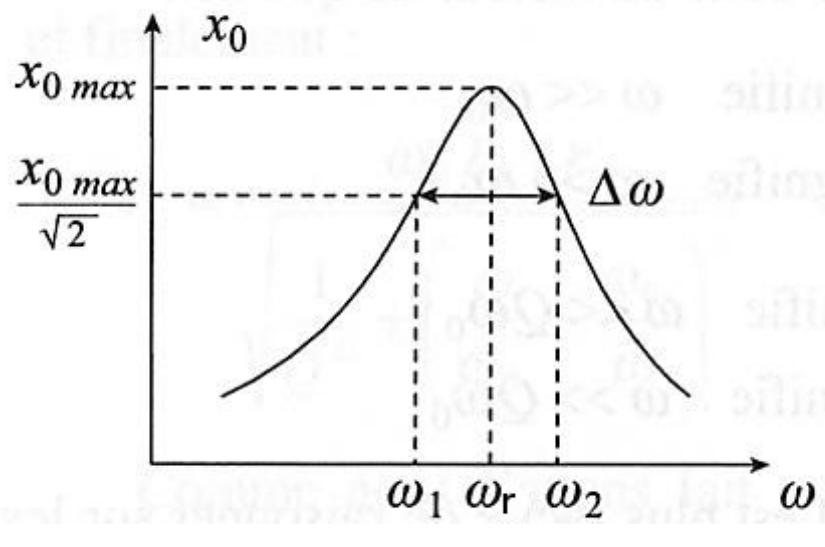
\includegraphics[width=\linewidth]{bandepass_moche}
    \end{center}
\end{minipage}

\section{Exemple d'oscillateur~: circuit RLC série en RSF}
\subsection{Présentation}

On étudie l'oscillateur amorti RLC série, dont le circuit en réel et en
complexes est le suivant~:
\begin{center}
    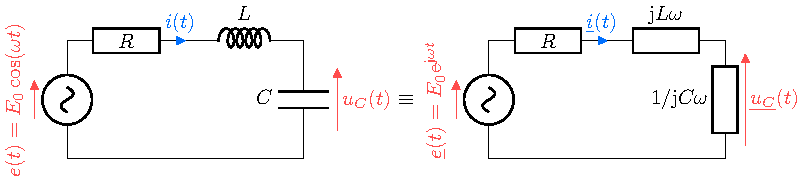
\includegraphics[width=\linewidth]{rlc_sinu}
\end{center}

\begin{rrapp}{Rappel}
    Pour un signal d'entrée $e(t) = E_0 \cos(\wt)$ les différentes tensions et
    intensités dans le circuit oscilleront \textbf{à la même pulsation $\w$}, et
    seront de la forme $u(t) = U\cos(\wt+\f_u) \qet i(t) = I\cos(\wt+\f_i)$ où
    $U$ et $\f_{u,i}$ sont deux constantes dépendant du système et de
    l'excitation $\w$.
\end{rrapp}

\subsection{Étude de l'intensité}
\begin{rdefi}{Situation initiale}
    \begin{minipage}{0.70\linewidth}
        Pour étudier le comportement de l'intensité, on va comme d'habitude se
        ramener à une seule maille avec une impédance équivalente
        \[\ul{Z}_{\eq} = \ul{Z}_R + \ul{Z}_L + \ul{Z}_C\]
    \end{minipage}
    \hfill
    \begin{minipage}{0.25\linewidth}
        \begin{center}
            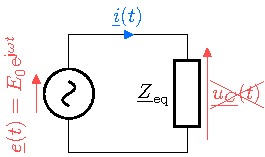
\includegraphics[width=\linewidth]{rlc_zeq}
        \end{center}
    \end{minipage}
\end{rdefi}
\vspace{-20pt}
\subsubsection{Équation}
\begin{rexem}{Développement}
    Avec l'impédance équivalente $\ul{Z_{\eq}}$, on a 
    \begin{align*}
        E = \ul{Z_{\eq}}\ul{I} &= \left( R + \jj L\w + \frac{1}{\jj C\w} \right)\\
        \Leftrightarrow
        \ul{I} &= \frac{E}{R + \jj \left( L\w - \dfrac{1}{C\w} \right)}\\
        \Leftrightarrow
        \ul{I} &= \frac{E/R}{1 + \jj \left( \dfrac{L}{R}\w  - \dfrac{1}{RC\w}\right)}
    \end{align*}
\end{rexem}
\begin{rdemo}{Méthode de calcul}
    Ici on a factorisé par $R$ pour avoir un numérateur homogène à une intensité, et
    un dénominateur adimensionné. On aimerait aller plus loin, et transformer les
    $\frac{L}{R}$ et $RC$ en expressions semblables à $\w$, en les reliant à $\w_0 =
    \frac{1}{\sqrt{LC}}$. Pour cela, on se rappelle la forme canonique de l'équation
    différentielle sur $i(t)$ du RLC~:
    \[
        \dv[2]{i}{t} + \frac{R}{L} \dv{i}{t} + \frac{1}{LC}i = 0
        \Leftrightarrow
        \dv[2]{i}{t} + \frac{\w_0}{Q} \dv{i}{t} + \w_0{}^2i = 0
    \]
    avec $\w_0$ la \textbf{pulsation propre} et $Q$ le \textbf{facteur de qualité},
    tels que
    \begin{gather*}
        \boxed{\w_0{}^2 = \frac{1}{LC}}
        \qet
        \frac{\w_0}{Q} = \frac{R}{L}
        \Leftrightarrow
        \boxed{Q = \frac{1}{R} \sqrt{\frac{L}{C}}}
    \end{gather*}
    Ainsi,
    \begin{gather*}
        \boxed{\frac{L}{R} = \frac{Q}{\w_0}}
        \qet
        Q\w_0 = \frac{1}{R} \sqrt{\frac{\cancel{L}}{C}} \frac{1}{\sqrt{\cancel{L}C}}
        \Leftrightarrow
        \boxed{ \frac{1}{RC} = Q\w_0}
    \end{gather*}
\end{rdemo}
\begin{rprop}{Résultat}
    On peut donc réécrire la fraction initiale~:
    \begin{gather*}
        \ul{I} = \frac{E/R}{1 + \jj \left( \dfrac{Q\w}{\w_0} - \dfrac{Q\w_0}{\w}
        \right)}
        \Leftrightarrow
        \boxed{
            \ul{I} = \frac{E/R}{1 + \jj Q \left(
                \dfrac{\w}{\w_0} - \dfrac{\w_0}{\w}
            \right)}}
    \end{gather*}
\end{rprop}

\subsubsection{Amplitude}

\begin{rprop}{Résultat}
    On trouve l'amplitude réelle en prenant le module, et comme en introduction
    cette amplitude dépend de la pulsation du système~:
    \[\boxed{
            I(\w)
            = \left| \ul{I} \right|
            = \frac{E_0/R}{\sqrt{1 + Q^2\left( \dfrac{\w}{\w_0} - \dfrac{\w_0}{\w}
            \right)^2}}
    }\]
\end{rprop}
\begin{rdemo}{Méthode}
    On trouve le maximum de cette amplitude quand le dénominateur est minimal,
    c'est-à-dire
    \begin{gather*}
        I(\w_r) = I_{\max}
        \Leftrightarrow
        1 + Q^2\left( \frac{\w_r}{\w_0} - \frac{\w_0}{\w_r} \right)^2 \text{minimal}\\
        \Leftrightarrow
        Q^2\left( \frac{\w_r}{\w_0} - \frac{\w_0}{\w_r} \right)^2 = 0
        \Leftrightarrow
        \boxed{\w_r = \w_0}
    \end{gather*}
\end{rdemo}
\begin{rror}{Conclusion}
    On trouve alors
    \[\boxed{
            I_{\max} = I(\w_0) = \frac{E_0}{R}
    }
    \qet
    \boxed{
        I\xrightarrow[\w\rightarrow0^+]{} 0}
    \qet
    \boxed{
        I\xrightarrow[\w\rightarrow+\infty]{} 0}
    \]
    De ce résultat, nous observons qu'il \textbf{n'y a pas de condition pour avoir
    résonance en intensité}, et que \textbf{la pulsation de résonance est la
    pulsation propre du système}.
\end{rror}

\vspace{-20pt}
\subsubsection{Phase}
\begin{rprop}{Résultat}
    Pour finir l'étude du système, il nous faut déterminer la phase en prenant
    l'argument de $\ul{I}$, en se souvenant que l'argument d'un rapport est la
    différence des arguments~:
    \begin{gather*}
        \f_i
            = \underbrace{\cancel{\arg(E_0/R)}}_{=0}
                - \arg \left( 1 + \jj Q \left(
                    \frac{\w}{\w_0} - \frac{\w_0}{\w}
                \right) \right)
        \Leftrightarrow
        \boxed{\tan\f_i = -Q\left( \frac{\w}{\w_0} - \frac{\w_0}{\w} \right)}
        \qavec
        \boxed{\f_i \in \left] - \frac{\pi}{2}\,; \frac{\pi}{2} \right[}
    \end{gather*}
    puisque $\cos\f_i > 0$ (la partie réelle est positive).
\end{rprop}
\begin{rror}{Conclusion}
    \[\tan\f_i \xrightarrow[\w\rightarrow0^+]{} +\infty \Rightarrow
        \boxed{\f_i \xrightarrow[\w\rightarrow0^+]{} +\pi/2}\]
    \[\tan(\f_i(\w_0)) = 0 \Rightarrow \boxed{\f_i(\w_0) = 0}\]
    \begin{center}
        \textbf{on peut détecter la résonance quand le déphasage entre
        $\ul{i}$ et $\ul{e}$ est nul.}
    \end{center}
    \[\tan\f_i \xrightarrow[\w\rightarrow+\infty]{} -\infty \Rightarrow
        \boxed{\f_i \xrightarrow[\w\rightarrow0^+]{} -\pi/2}\]
\end{rror}

\vspace{-20pt}
\subsubsection{Facteur de qualité et bande passante}
\begin{rdefi}{Définition}
    Nous avons déterminé l'amplitude et la phase du signal, ainsi que la
    pulsation de résonance. Pour finir de caractériser la résonance, il ne reste
    qu'à déterminer la bande passante. On cherche donc les pulsations de coupure
    telles que $I(\w) = \frac{I_{\max}}{\sqrt{2}}$.
\end{rdefi}
\begin{rimpl}{Implication}
    \vspace{-10pt}
    \begin{gather*}
        I(\w) = \frac{I_{\max}}{\sqrt{2}}
        \Leftrightarrow
        \frac{E_0/R}{\sqrt{1 + Q^2\left( \frac{\w}{\w_0} - \frac{\w_0}{\w}
                \right)^2}}
            =
            \frac{E_0/R}{\sqrt{2}}
            \Leftrightarrow
            \boxed{Q^2\left( \frac{\w}{\w_0} - \frac{\w_0}{\w} \right)^2 = 1}
    \end{gather*}
\end{rimpl}
\begin{rexem}{Calculs}
    On prend la racine carrée de cette équation, \textbf{en prenant les deux
    solutions possibles}~:
    \begin{align*}
        Q\left( \frac{\w}{\w_0} - \frac{\w_0}{\w} \right) = -1
        &\qet
        Q\left( \frac{\w}{\w_0} - \frac{\w_0}{\w} \right) = 1\\
        \Leftrightarrow
        \left( \frac{\w}{\w_0} - \frac{\w_0}{\w} \right)\times \w\w_0 =
            - \frac{\w\w_0}{Q}
        &\qet
        \left( \frac{\w}{\w_0} - \frac{\w_0}{\w} \right)\times \w\w_0 =
            \frac{\w\w_0}{Q}\\
        \Leftrightarrow
        \w^2 - \w_0{}^2 = -\frac{\w\w_0}{Q}
        &\qet
        \w^2 - \w_0{}^2 = \frac{\w\w_0}{Q}\\
        \Leftrightarrow
        \boxed{
        \w^2 + \frac{\w_0}{Q}\w - \w_0{}^2 = 0}
        &\qet
        \boxed{
        \w^2 - \frac{\w_0}{Q}\w - \w_0{}^2 = 0}\\
        \Rightarrow
        \Delta = &\frac{\w_0{}^2}{Q} + 4\w_0{}^2\\
        \Leftrightarrow
        \Delta = &\frac{\w_0{}^2}{Q^2} \left( 1 + 4Q^2 \right)\\
        \Rightarrow
        \w_{1,\pm} = -\frac{\w_0}{2Q} \pm \frac{\w_0}{2Q} \sqrt{1+4Q^2}
        &\qet
        \w_{2,\pm} = \frac{\w_0}{2Q} \pm \frac{\w_0}{2Q} \sqrt{1+4Q^2}\\
        \Leftrightarrow
        \w_{1,\pm} = \frac{\w_0}{2Q} \left(-1 \pm \sqrt{1+4Q^2}\right)
        &\qet
        \w_{2,\pm} = \frac{\w_0}{2Q} \left(1 \pm \sqrt{1+4Q^2}\right)
    \end{align*}
    De ces quatre racines, seules deux sont positives~: la solution avec $-1 -
    \sqrt{1+4Q^2}$ est évidemment négative, et celle avec $1 - \sqrt{1+4Q^2}$
    également. Ainsi, il ne nous reste que
    \begin{gather*}
        \w_1 = \frac{\w_0}{2Q} \left( \sqrt{1+4Q^2}-1 \right)
        \qet
        \w_1 = \frac{\w_0}{2Q} \left( \sqrt{1+4Q^2}+1 \right)
    \end{gather*}
\end{rexem}

\begin{rprop}{Résultat}
    Il ne reste qu'à calculer la différence pour avoir la bande passante~:
    \begin{gather*}
        \boxed{\D\w = \w_2 - \w_1 = \frac{\w_0}{Q}
            \Leftrightarrow
            Q = \frac{\w_0}{\D\w}
        }
    \end{gather*}
    ce qui est également une \textbf{nouvelle définition de $Q$}~! En effet, cette
    égalité traduit le fait qu'à haut facteur de qualité, la bande passante est très
    faible, ou que \textbf{l'acuité de la résonance est élevée}.
\end{rprop}

\vspace{-20pt}
\begin{center}
    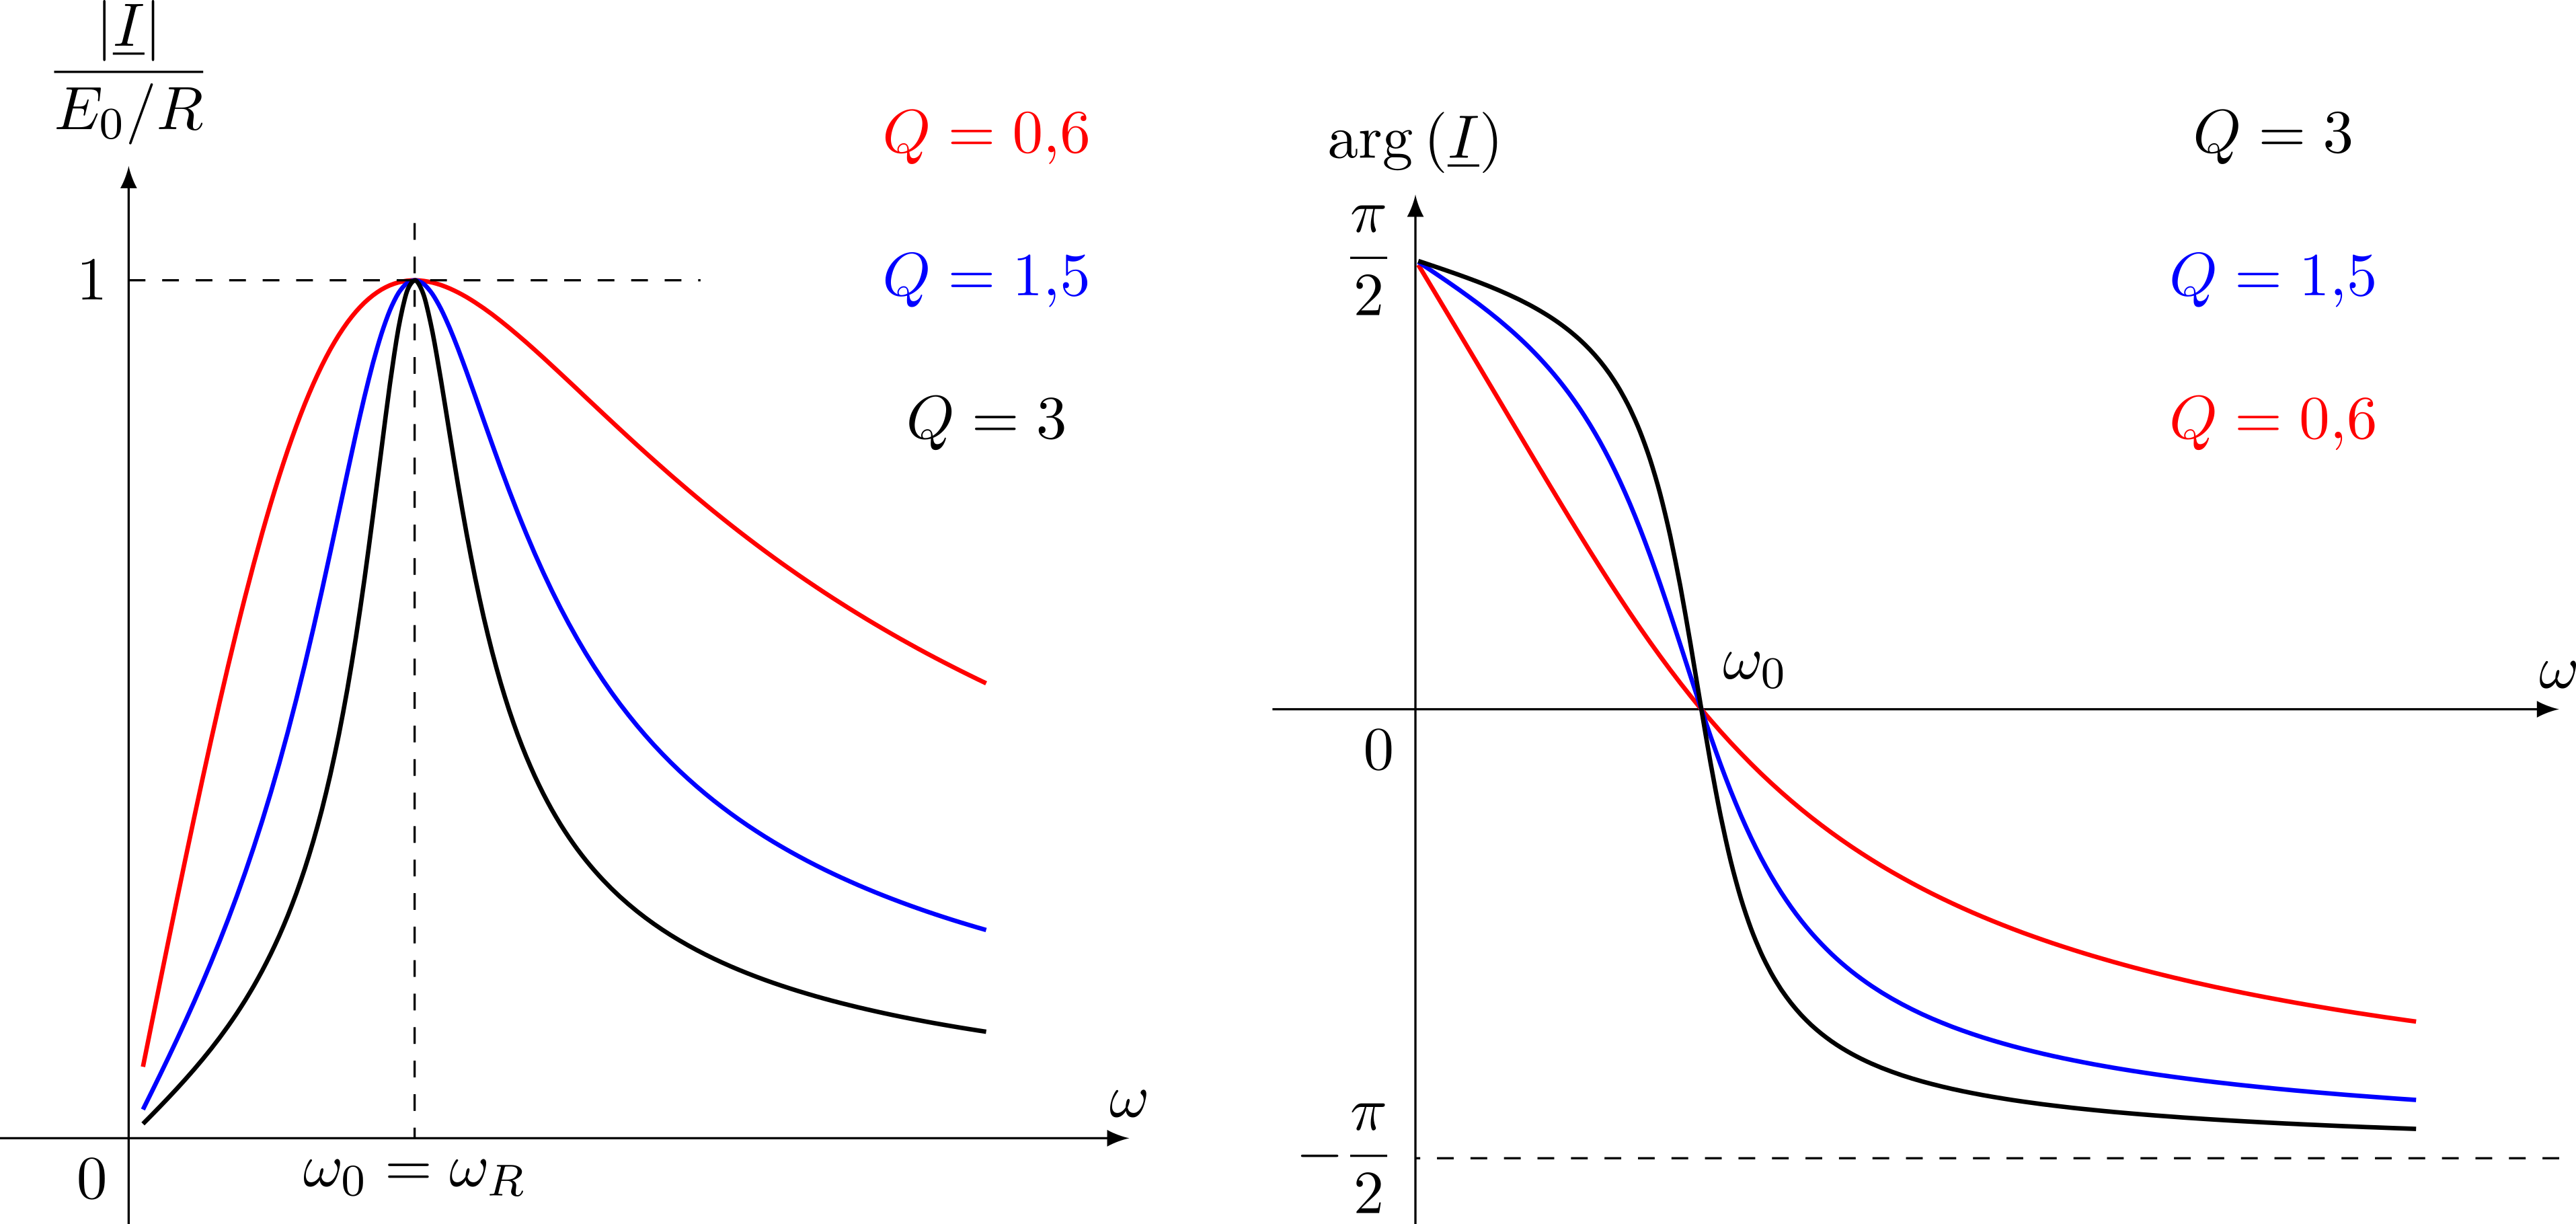
\includegraphics[width=.8\linewidth]{rlc_i-ampphase}
\end{center}

\subsection{Étude de la tension}
On repart du circuit en complexes, avec $\ul{u_C}(t) = \ul{U}\exr^{\jj\wt}$ et
$\ul{e}(t) = E\exr^{\jj\wt}$, et on applique le pont diviseur de tension

\subsubsection{Amplitude complexe}
\begin{rdefi}{Situation initiale}
    \vspace{-20pt}
    \begin{minipage}{0.40\linewidth}
        \begin{center}
            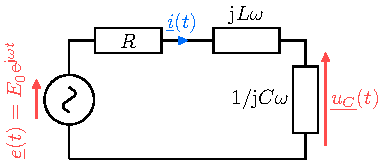
\includegraphics[width=\linewidth]{rlc_u-circ}
        \end{center}
    \end{minipage}
    \hfill
    \begin{minipage}{0.60\linewidth}
        \begin{lprop}{Résultat}
            \begin{gather*}
                \ul{U} = \frac{1/\jj C\w}{R + \jj L\w + 1/\jj C\w}E
                \Leftrightarrow
                \ul{U} = \frac{E}{1 - (LC\w)^2 + \jj RC\w}\\
                \Leftrightarrow
                \boxed{
                    \ul{U}
                        = \frac{E}{1 -
                                    \left( \dfrac{\w}{\w_0} \right)^2 +
                                    \jj\dfrac{\w}{Q\w_0}}
                    }
            \end{gather*}
        \end{lprop}
    \end{minipage}
\end{rdefi}
\begin{rdemo}{Méthode de calcul}
    Ici encore, on a factorisé par $1/\jj C\w$ pour avoir un numérateur homogène
    à une tension et
    un dénominateur adimensionné d'abord. Ensuite puis pour aller plus loin, on
    transformer les $LC$ et $RC$ en expressions semblables à $\w$, en les
    reliant à $\w_0$. On a comme précédemment
    \begin{gather*}
        \boxed{\w_0{}^2 = \frac{1}{LC}}
        \qet
        \boxed{Q = \frac{1}{R} \sqrt{\frac{L}{C}}}
        \qdonc
        Q\w_0 = \frac{1}{R} \sqrt{\frac{\cancel{L}}{C}} \frac{1}{\sqrt{\cancel{L}C}}
        \Leftrightarrow
        \boxed{ \frac{1}{RC} = Q\w_0}
    \end{gather*}
\end{rdemo}

\subsubsection{Amplitude réelle et condition de résonance}
\begin{rprop}{Résultat}
    On trouve l'amplitude réelle en prenant le module, et comme en introduction
    cette amplitude dépend de la pulsation du système~:
    \[\boxed{
            U(\w)
            = \left| \ul{U} \right|
            = \frac{E_0}{
                \sqrt{\left( 1 - \left(\dfrac{\w}{\w_0}\right)^2 \right)^2
                + \left(\dfrac{\w}{Q\w_0}\right)^2}}
    }\]
\end{rprop}
\begin{rdemo}{Méthode}
    On trouve le maximum de cette amplitude quand le dénominateur est
    \textbf{non nul} et minimal, c'est-à-dire
    \begin{gather*}
        U(\w_r) = U_{\max}
        \Leftrightarrow
        \left( 1 - \left(\dfrac{\w}{\w_0}\right)^2 \right)^2
                + \left(\dfrac{\w}{Q\w_0}\right)^2 \text{minimal}
    \end{gather*}
    Soit $X = \left( \dfrac{\w}{\w_0} \right)^2$, et $f(X) = \left(1 - X\right)^2
    + \dfrac{X}{Q^2}$, la fonction que l'on cherche à minimiser~: on cherche donc
    quand est-ce que sa dérivée est nulle, c'est-à-dire
    \begin{gather*}
        f'(X_r) = 0
        \Leftrightarrow
        -2 \left( 1-X_r \right) + \frac{1}{Q^2} = 0
        \Leftrightarrow
        X_r-1 = - \frac{1}{2Q^2}
        \Leftrightarrow
        X_r = 1 - \frac{1}{2Q^2}\\
        \Leftrightarrow
        \boxed{
        \w_r = \w_0 \sqrt{1 - \frac{1}{2Q^2}}}
    \end{gather*}
    ce qui n'est défini \textbf{que si} $Q > \dfrac{1}{\sqrt{2}}$.
\end{rdemo}
\begin{rror}{Conclusion}
    On trouve alors~:
    \begin{itemize}[leftmargin=60pt]
        \item[$\mathbf{Q \leq 1/\sqrt{2}}$] : \textbf{pas de résonance},
            l'amplitude est maximale pour
            \[\boxed{\w = 0 \qet U(0) = E_0}\]
        \item[$\mathbf{Q > 1/\sqrt{2}}$] : l'amplitude est maximale pour
            \[\boxed{\w_r = \w_0 \sqrt{1 - \frac{1}{2Q^2}} < \w_0}
                \qet
                \boxed{U(\w_r) = \frac{QE}{\sqrt{1 - \frac{1}{4Q^2}}}}
            \]
        \item[$\mathbf{Q > 5}$] :
            \[\boxed{\w_r \approx \w_0}
                \qet
                \boxed{U(\w_r) \approx QE}
            \]
    \end{itemize}
    De ce résultat, nous observons qu'il \textbf{n'y a pas toujours résonance en
    tension}, et que \textbf{la résonance est d'autant aiguë que $\mathbf{Q}$
    est élevé}.
\end{rror}

\subsubsection{Phase}
\begin{rprop}{Résultat}
    Ici aussi, on détermine la phase en prenant l'argument de l'amplitude complexe~:
    \begin{gather*}
        \f_u = \underbrace{\cancel{\arg(E_0)}}_{=0}
            - \arg \left( 1 - \left(\frac{\w}{\w_0}\right)^2 + \jj \frac{\w}{Q\w_0}\right)
        \Leftrightarrow
        \boxed{
            \tan\f_u = -\frac{\w}{Q\w_0\left(
                1 - \left( \frac{\w}{\w_0}
            \right)^2\right)}
        }
        \qavec
        \boxed{
            \f_u \in \left] -\pi\,; 0 \right[}
    \end{gather*}
\end{rprop}
\begin{rror}{Conclusion}
    \[\tan\f_u \xrightarrow[\w\rightarrow0^+]{} 0
        \Rightarrow
        \boxed{\f_u \xrightarrow[\w\rightarrow0^+]{} 0}
    \]
    \[\tan(\f_u(\w_0)) \longrightarrow -\infty
        \Rightarrow
        \boxed{\f_u(\w_0) = - \frac{\pi}{2}}
    \]
    \[\tan\f_u \xrightarrow[\w\rightarrow+\infty]{} 0
        \Rightarrow
        \boxed{\f_u \xrightarrow[\w\rightarrow0^+]{} - \pi}
    \]
\end{rror}

\begin{center}
    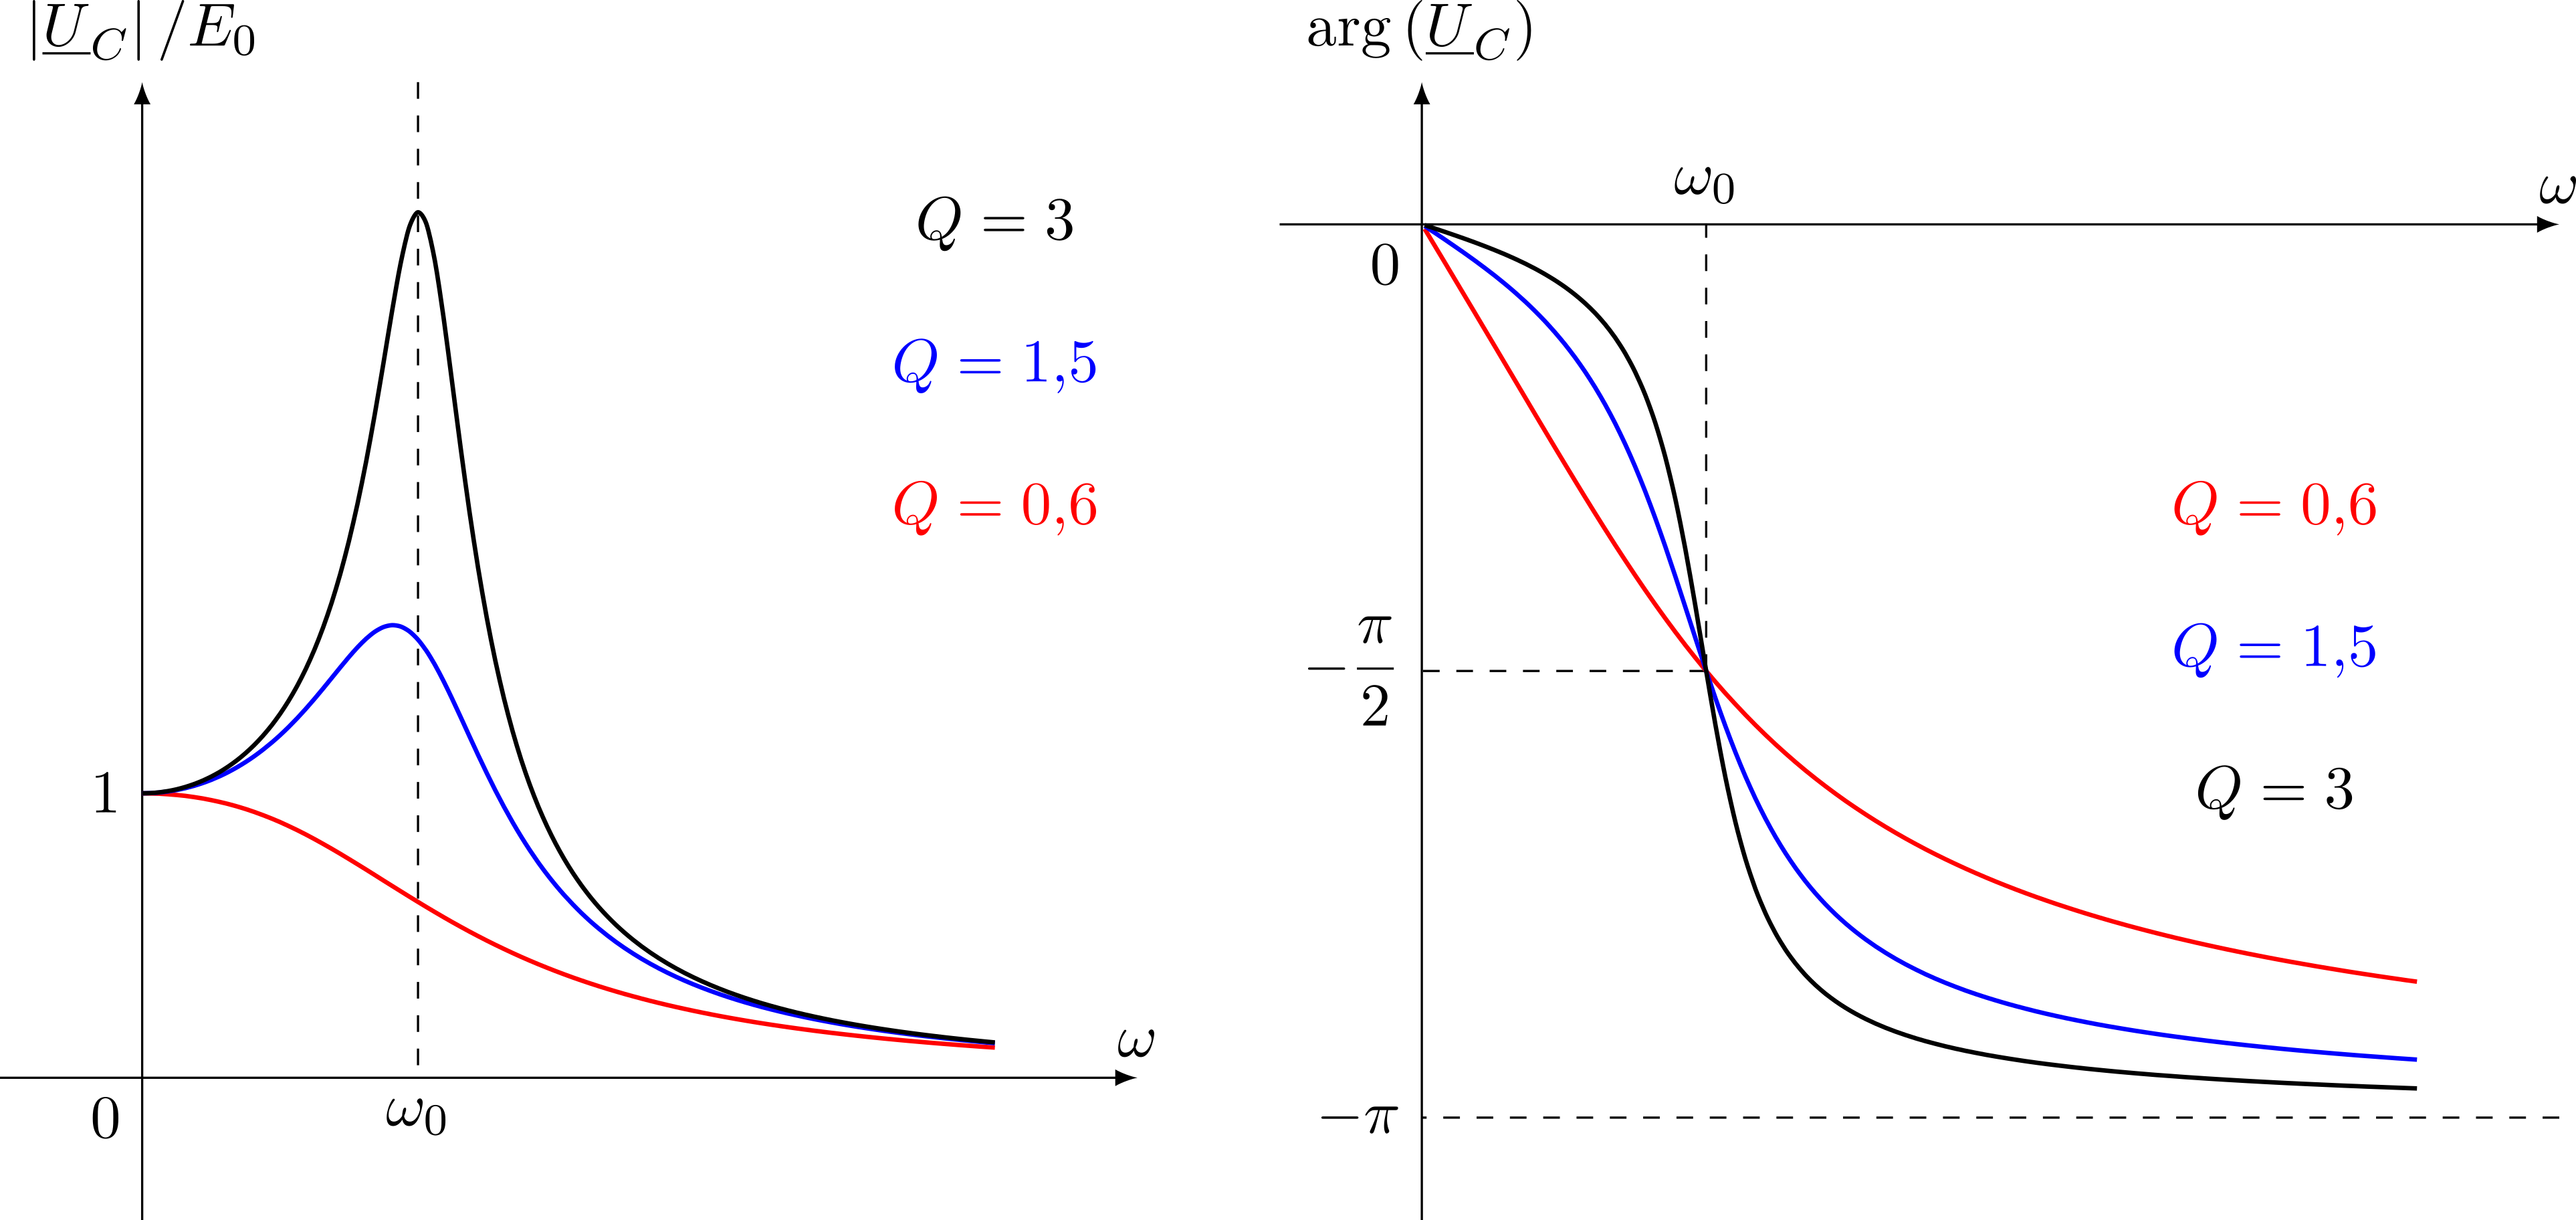
\includegraphics[width=0.9\linewidth]{rlc_u-ampphase}
\end{center}

\section{Exemple d'un oscillateur mécanique en RSF}
\subsection{Présentation}
\begin{rdefi}{Situation initiale}
    \begin{description}
        \item[Système] : point matériel $M$ de masse $m$ relié à un ressort
            horizontal \textbf{idéal}.
        \item[Référentiel] : $\Rc_{\rm sol} (O,x,y,t)$~;
    \end{description}

    \centers{\fbox{Soit $x = \ell - \ell_0$ la position de la masse}}\bigbreak

    \begin{minipage}{0.55\linewidth}
        \textbf{Bilan des forces}~:
        \begin{enumerate}
            \item Poids $\Pf = -mg\uy$~;
            \item Réaction du support $\vv{R} = R\uy$~;
            \item Force de rappel du ressort $\vv*{F}{\rm ressort} = -kx\ux$~;
            \item Force de frottement fluide $\vv*{F}{\rm frott} = -\alpha\vf$~;
            \item \textbf{Force excitatrice} $\ff_e = F_0\cos(\wt)\ux$.
        \end{enumerate}
    \end{minipage}
    \begin{minipage}{0.45\linewidth}
        \begin{center}
            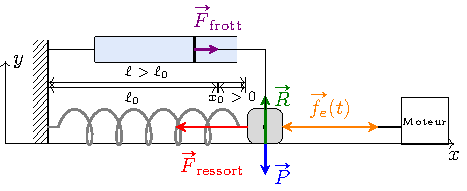
\includegraphics[width=\linewidth]{ressort-horiz}
        \end{center}
    \end{minipage}

\end{rdefi}

\subsection{Étude de l'élongation}
\subsubsection{Équation}

\begin{rexem}{Calculs}
    Avec le PFD~:
    \begin{gather*}
        m\af = \Pf + \vv{R} + \Ff_{\rm ressort} + \Ff_{\rm frott} +\ff_e\\
        \Leftrightarrow m\left(
            \begin{array}{c}
                \dv[2]{x}{t}\\
                0
            \end{array}
        \right)
        =
        \left(
            \begin{array}{c}
                -kx -\alpha v + F_0\cos(\wt)\\
                -mg + R
            \end{array}
        \right)
    \end{gather*}
    La projection sur $\uy$ montre que la réaction du support compense le poids.
    Sur l'axe $\ux$ on trouve
    \begin{gather*}
        m \dv[2]{x}{t} + \alpha \dv{x}{t} + kx = F_0\cos(\wt)
        \Leftrightarrow
        \boxed{\ddot{x} + \frac{\w_0}{Q}\dot{x} + \w_0{}^2x =
            \frac{F_0}{m}\cos(\wt)}\\
        \qavec
        \boxed{\w_0 = \sqrt{\frac{k}{m}}}
        \qet
        Q = \frac{\sqrt{km}}{\alpha}
    \end{gather*}
\end{rexem}
\begin{rprop}{Résultat}
    En passant en complexes,
    \begin{gather*}
        \ul{X} = \frac{F_0/m}{\w_0{}^2 - \w^2 + \jj \frac{\w\w_0}{Q}}
        \Leftrightarrow
        \boxed{
        \ul{X} = \frac{F_0}{m\w_0{}^2}\frac{1}{1 -
                                    \left( \dfrac{\w}{\w_0} \right)^2 +
                                    \jj\dfrac{\w}{Q\w_0}}
                }
    \end{gather*}
\end{rprop}

\subsubsection{Amplitude réelle et condition de résonance}
\begin{rprop}{Résultat}
    On trouve
    \begin{gather*}
        \boxed{
        X(\w)
            = \left| \ul{X} \right|
            = \frac{F_0}{m\w_0{}^2}\frac{1}{
                    \sqrt{\left( 1 - \left(\dfrac{\w}{\w_0}\right)^2 \right)^2
                    + \left(\dfrac{\w}{Q\w_0}\right)^2}}
        }
    \end{gather*}
    Elle est maximale quand le dénominateur est minimal. Après calcul, on retrouve
    les résultats de l'excitation en tension~:
\end{rprop}
\begin{rror}{Conclusion}
    On trouve alors~:
    \begin{itemize}[leftmargin=60pt]
        \item[$\mathbf{Q \leq 1/\sqrt{2}}$] : l'amplitude est maximale pour
            \[\boxed{\w = 0 \qet X(0) = \frac{F_0}{m\w_0{}^2}}\]
        \item[$\mathbf{Q > 1/\sqrt{2}}$] : l'amplitude est maximale pour
            \[\boxed{\w_r = \w_0 \sqrt{1 - \frac{1}{2Q^2}} < \w_0}
                \qet
                \boxed{X(\w_r) = \frac{F_0}{m\w_0{}^2}
                    \frac{Q}{\sqrt{1 - \frac{1}{4Q^2}}}}
            \]
        \item[$\mathbf{Q > 5}$] :
            \[\boxed{\w_r \approx \w_0}
                \qet
                \boxed{X(\w_r) \approx QF_0/K}
            \]
    \end{itemize}
    De ce résultat, nous observons qu'il \textbf{n'y a pas toujours résonance en
    élongation}, et que \textbf{la résonance est d'autant aiguë que $\mathbf{Q}$
    est élevé}.
\end{rror}

Vous trouverez ici\footnote{\href{http://www.sciences.univ-nantes.fr/sites/genevieve\_tulloue/Meca/Oscillateurs/ressort\_rsf.php?typanim=Javascript}{http://www.sciences.univ-nantes.fr/sites/genevieve\_tulloue/Meca/Oscillateurs/ressort\_rsf.php?typanim=Javascript}} une animation interactive d'un système similaire avec un
ressort vertical.

\subsection{Résonance en vitesse}
\subsubsection{Équation}

\begin{rdefi}{\small Définition}
    On définit
    \[v(t) = \dv{x}{t} \Leftrightarrow \ul{V} = \jj\w\ul{X}\]
\end{rdefi}
D'où
\begin{rexem}{Calculs}
    \begin{gather*}
        \ul{V}
            = \jj\w\ul{X}
            = \frac{F}{m\w_0} \frac{\jj\w}{\w_0 \left( 1 -
                \left( \dfrac{\w}{\w_0} \right)^2 + \jj\dfrac{\w}{Q\w_0} \right)}
            = \frac{F}{m\w_0} \frac{\w}{-\jj \left( \w_0 - \dfrac{\w^2}{\w_0} +
                \jj \dfrac{\w}{Q} \right)}\\
        \Leftrightarrow
        \ul{V}
            = \frac{F}{m\w_0} \underbrace{\cancel{\frac{\w}{\w}}}_{=1}
                \frac{1}{-\jj \dfrac{\w_0}{\w} +\jj \dfrac{\w}{\w_0} - \jj^2
                \dfrac{1}{Q}}
            = \frac{F}{m\dfrac{\w_0}{Q}} \frac{1}{1 + \jj Q \left(
                \dfrac{\w}{\w_0} - \dfrac{\w_0}{\w}\right)}
    \end{gather*}
\end{rexem}
\begin{rprop}{Résultat}
    Ainsi,
    \begin{equation*}
        \boxed{
        \ul{V} = \frac{F_0}{\alpha} \frac{1}{1 + \jj Q \left(
                \dfrac{\w}{\w_0} - \dfrac{\w_0}{\w}\right)}}
        \quad\text{car}\quad
        m \frac{\w_0}{Q} = \alpha
    \end{equation*}
\end{rprop}
\begin{rror}{Conclusion}
    On trouve alors
    \[\boxed{
            V_{\max} = V(\w_0) = \frac{F_0}{\alpha}
    }
    \qet
    \boxed{
        V\xrightarrow[\w\rightarrow0^+]{} 0}
    \qet
    \boxed{
        V\xrightarrow[\w\rightarrow+\infty]{} 0}
    \]
    De ce résultat, nous observons qu'il \textbf{n'y a pas de condition pour avoir
    résonance en intensité}, et que \textbf{la pulsation de résonance est la
    pulsation propre du système}.
\end{rror}
%On retrouve également $Q = \w_0/\D\w$ avec $\f(\w_r) = 0$.

\vspace{-25pt}
\section{Synthèse}
\begin{ror}[label=ror:oscrsf_synth,
    tabularx*={\renewcommand{\arraystretch}{1.8}}{M{3cm}|Y|Y}, hand]
    {synthèse résonances}
    \textbf{Électricité} & Intensité & Tension
    \\\hdashline
    \textbf{Mécanique} & Vitesse & Élongation
    \\\hline
    \textbf{Existence} & Toujours & $Q > 1/\sqrt{2}$
    \\\hline
    \textbf{Pulsation de résonance} & $\w_0$ & $\w_r \lesssim \w_0$
    \\\hdashline
    \textbf{Largeur de résonance} & $\D\w = \dfrac{\w_0}{Q}$ & $\D\w \approx
    \dfrac{\w_0}{Q}$
    \\\hline
    \textbf{Aspects à $\w_r$} & Maximum d'amplitude\smallbreak Déphasage nul, $\f = 0$ &
    Maximum d'amplitude
    \\\hdashline
    \textbf{Aspects à $\w_0$} & Résonance & Sortie = $Q\times$entrée\smallbreak
    Quadrature de phase, $\f = -\dfrac{\pi}{2}$
    \\\hline
    \textbf{Courbes d'amplitude} & 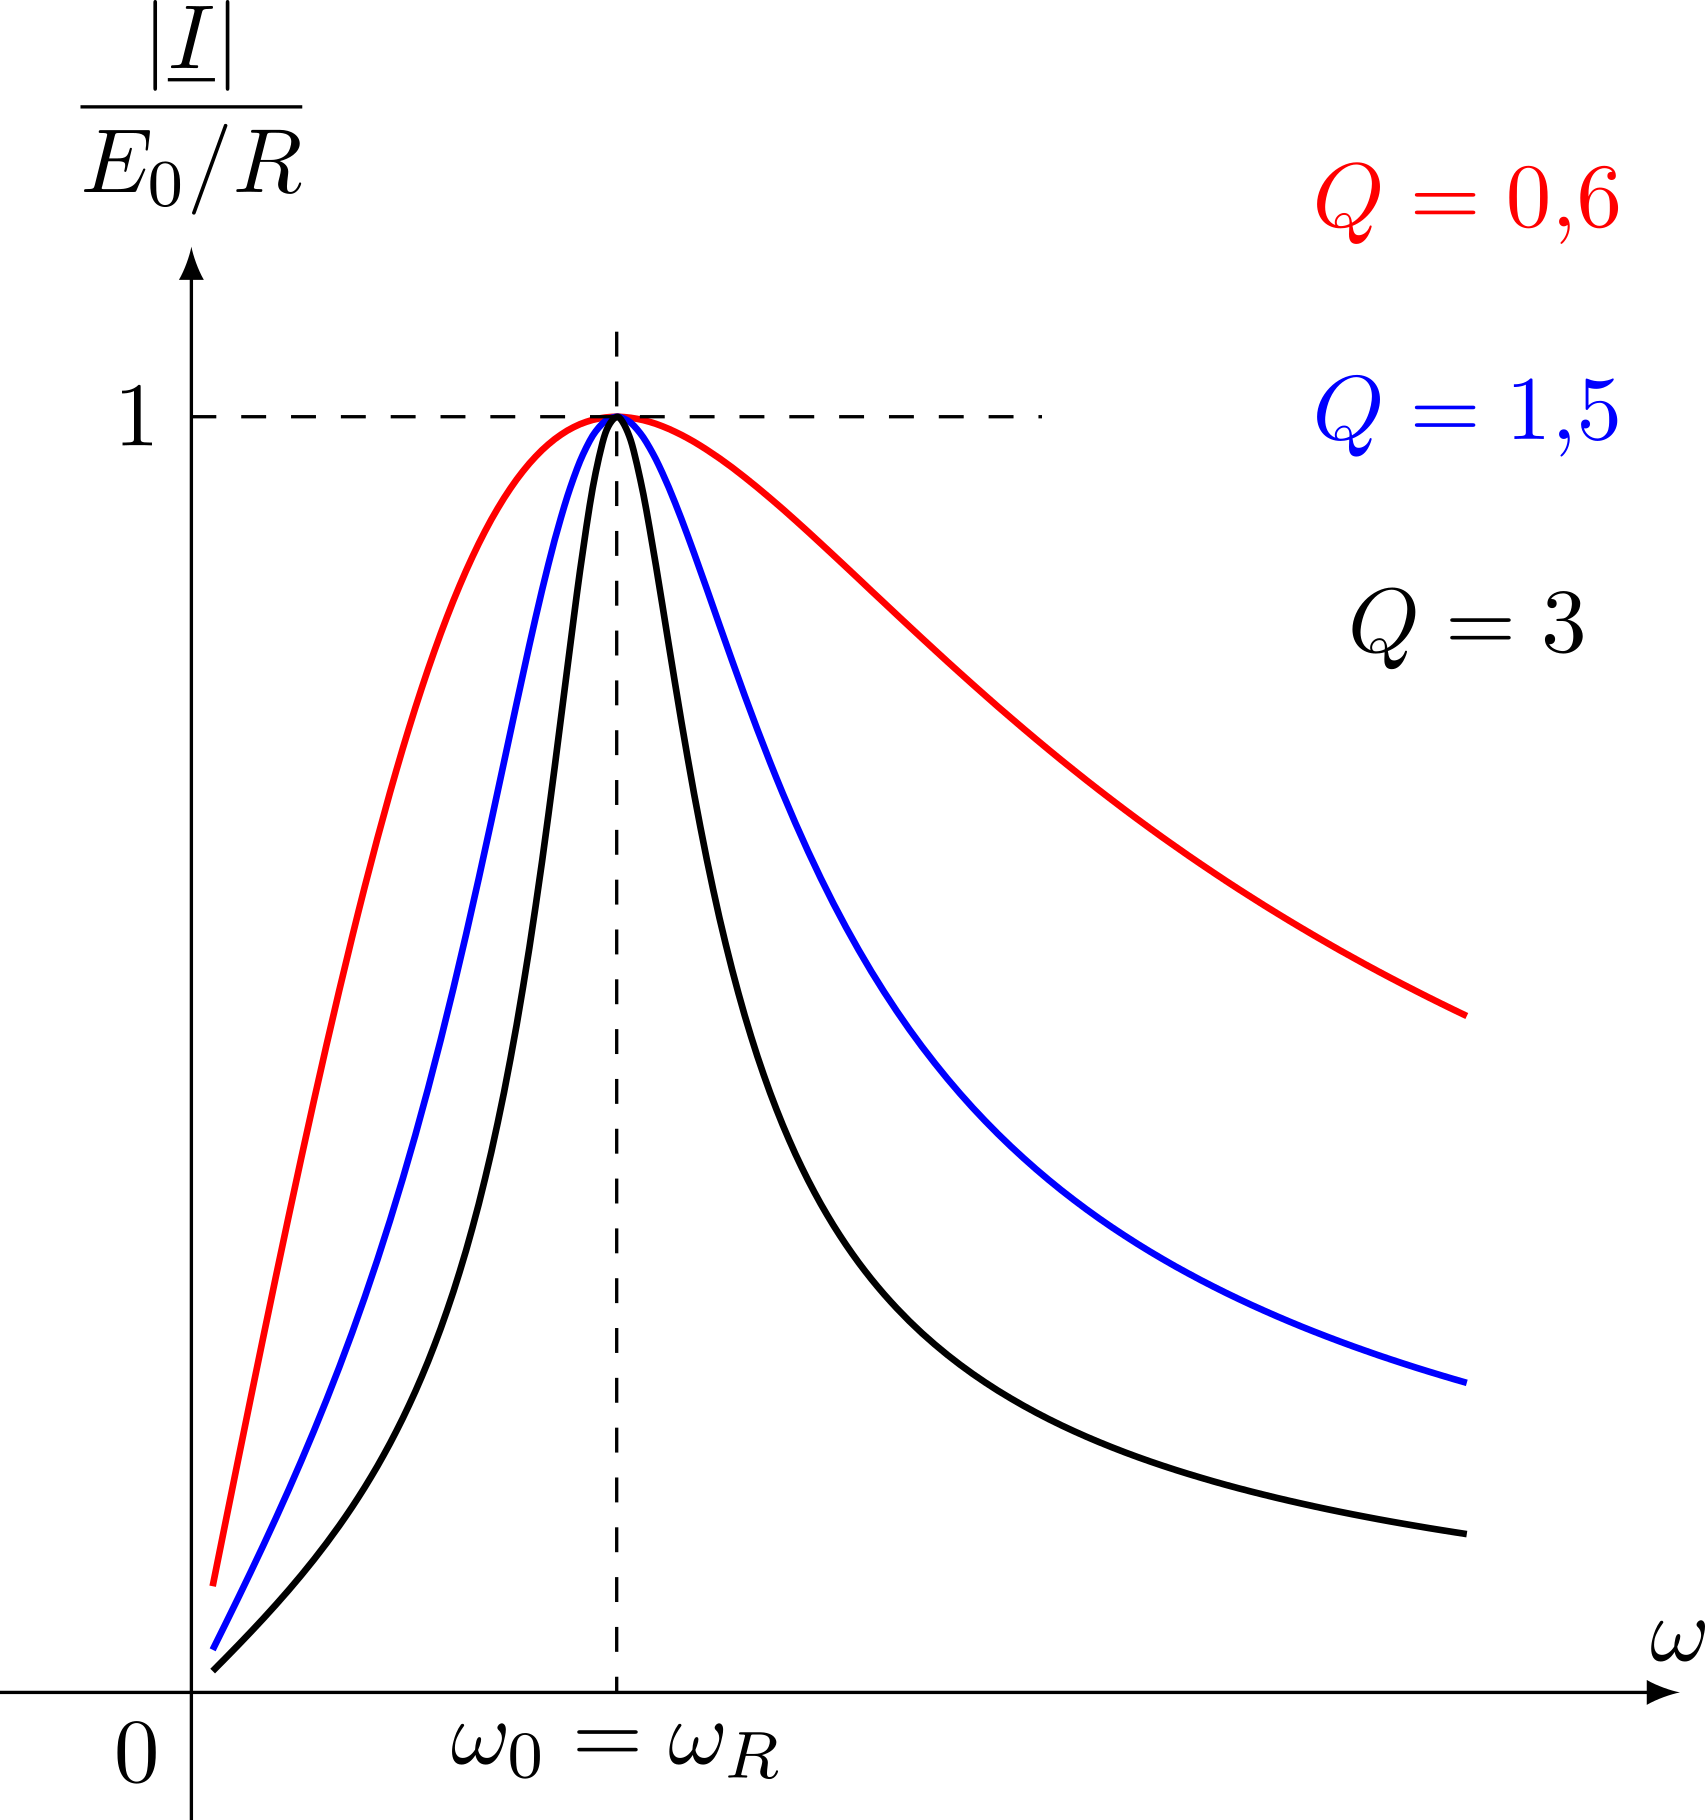
\includegraphics[width=.6\linewidth]{rlc_i-amp}
                                 & 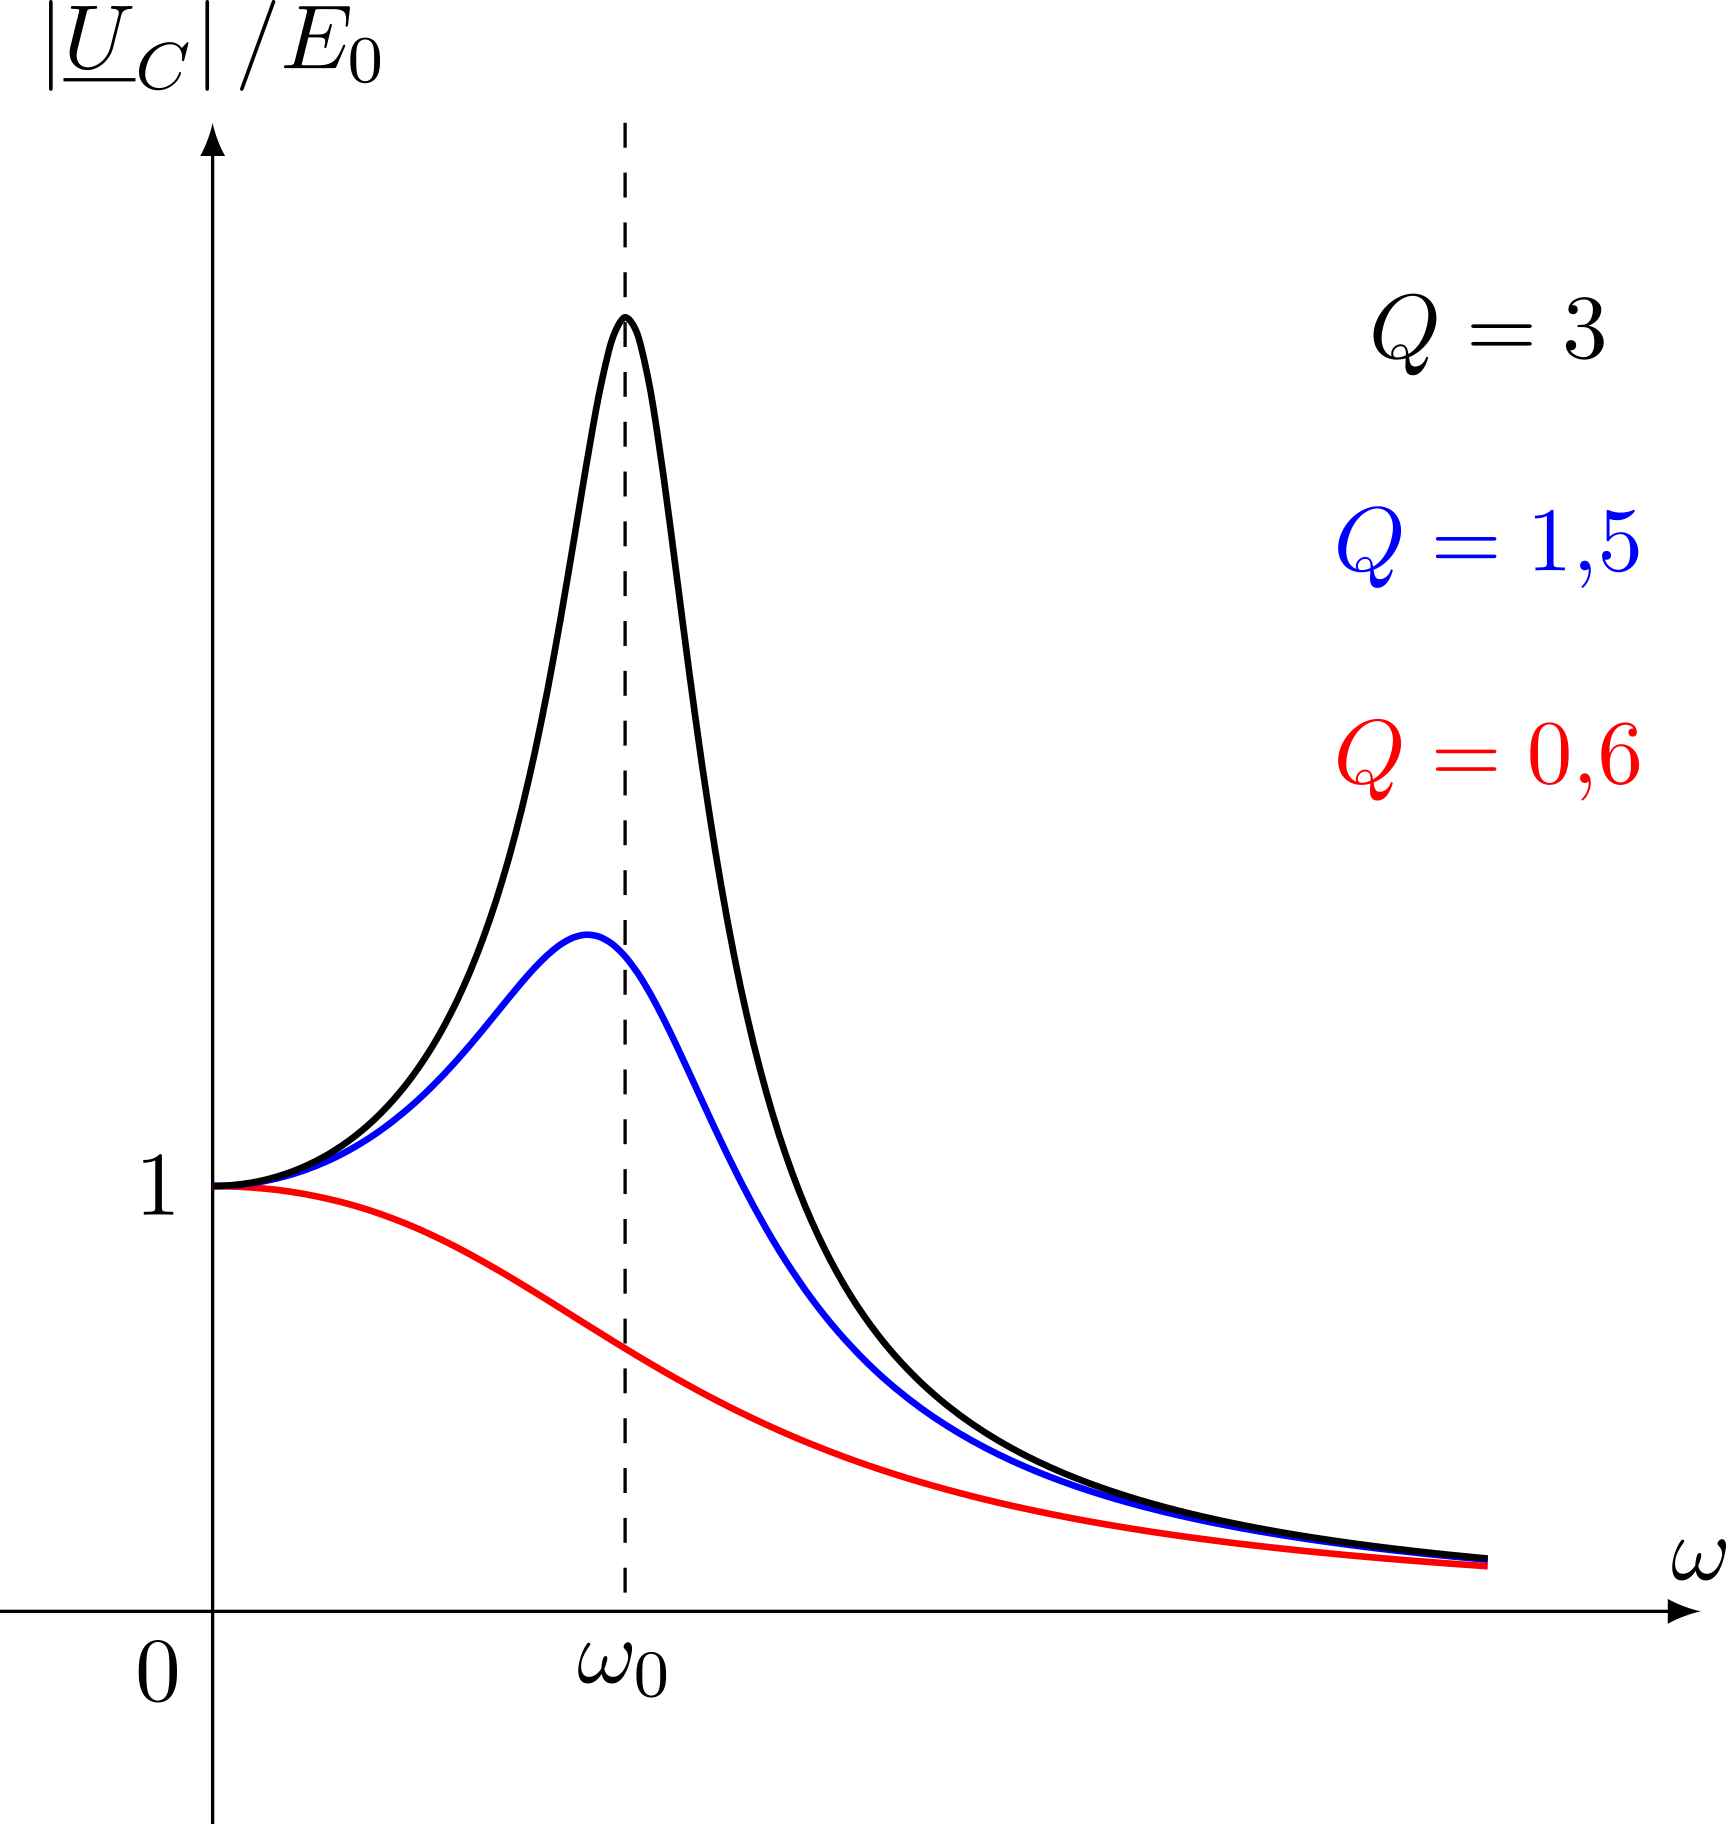
\includegraphics[width=.6\linewidth]{rlc_u-amp}
    \\\hdashline
    \textbf{Courbes de phase} & 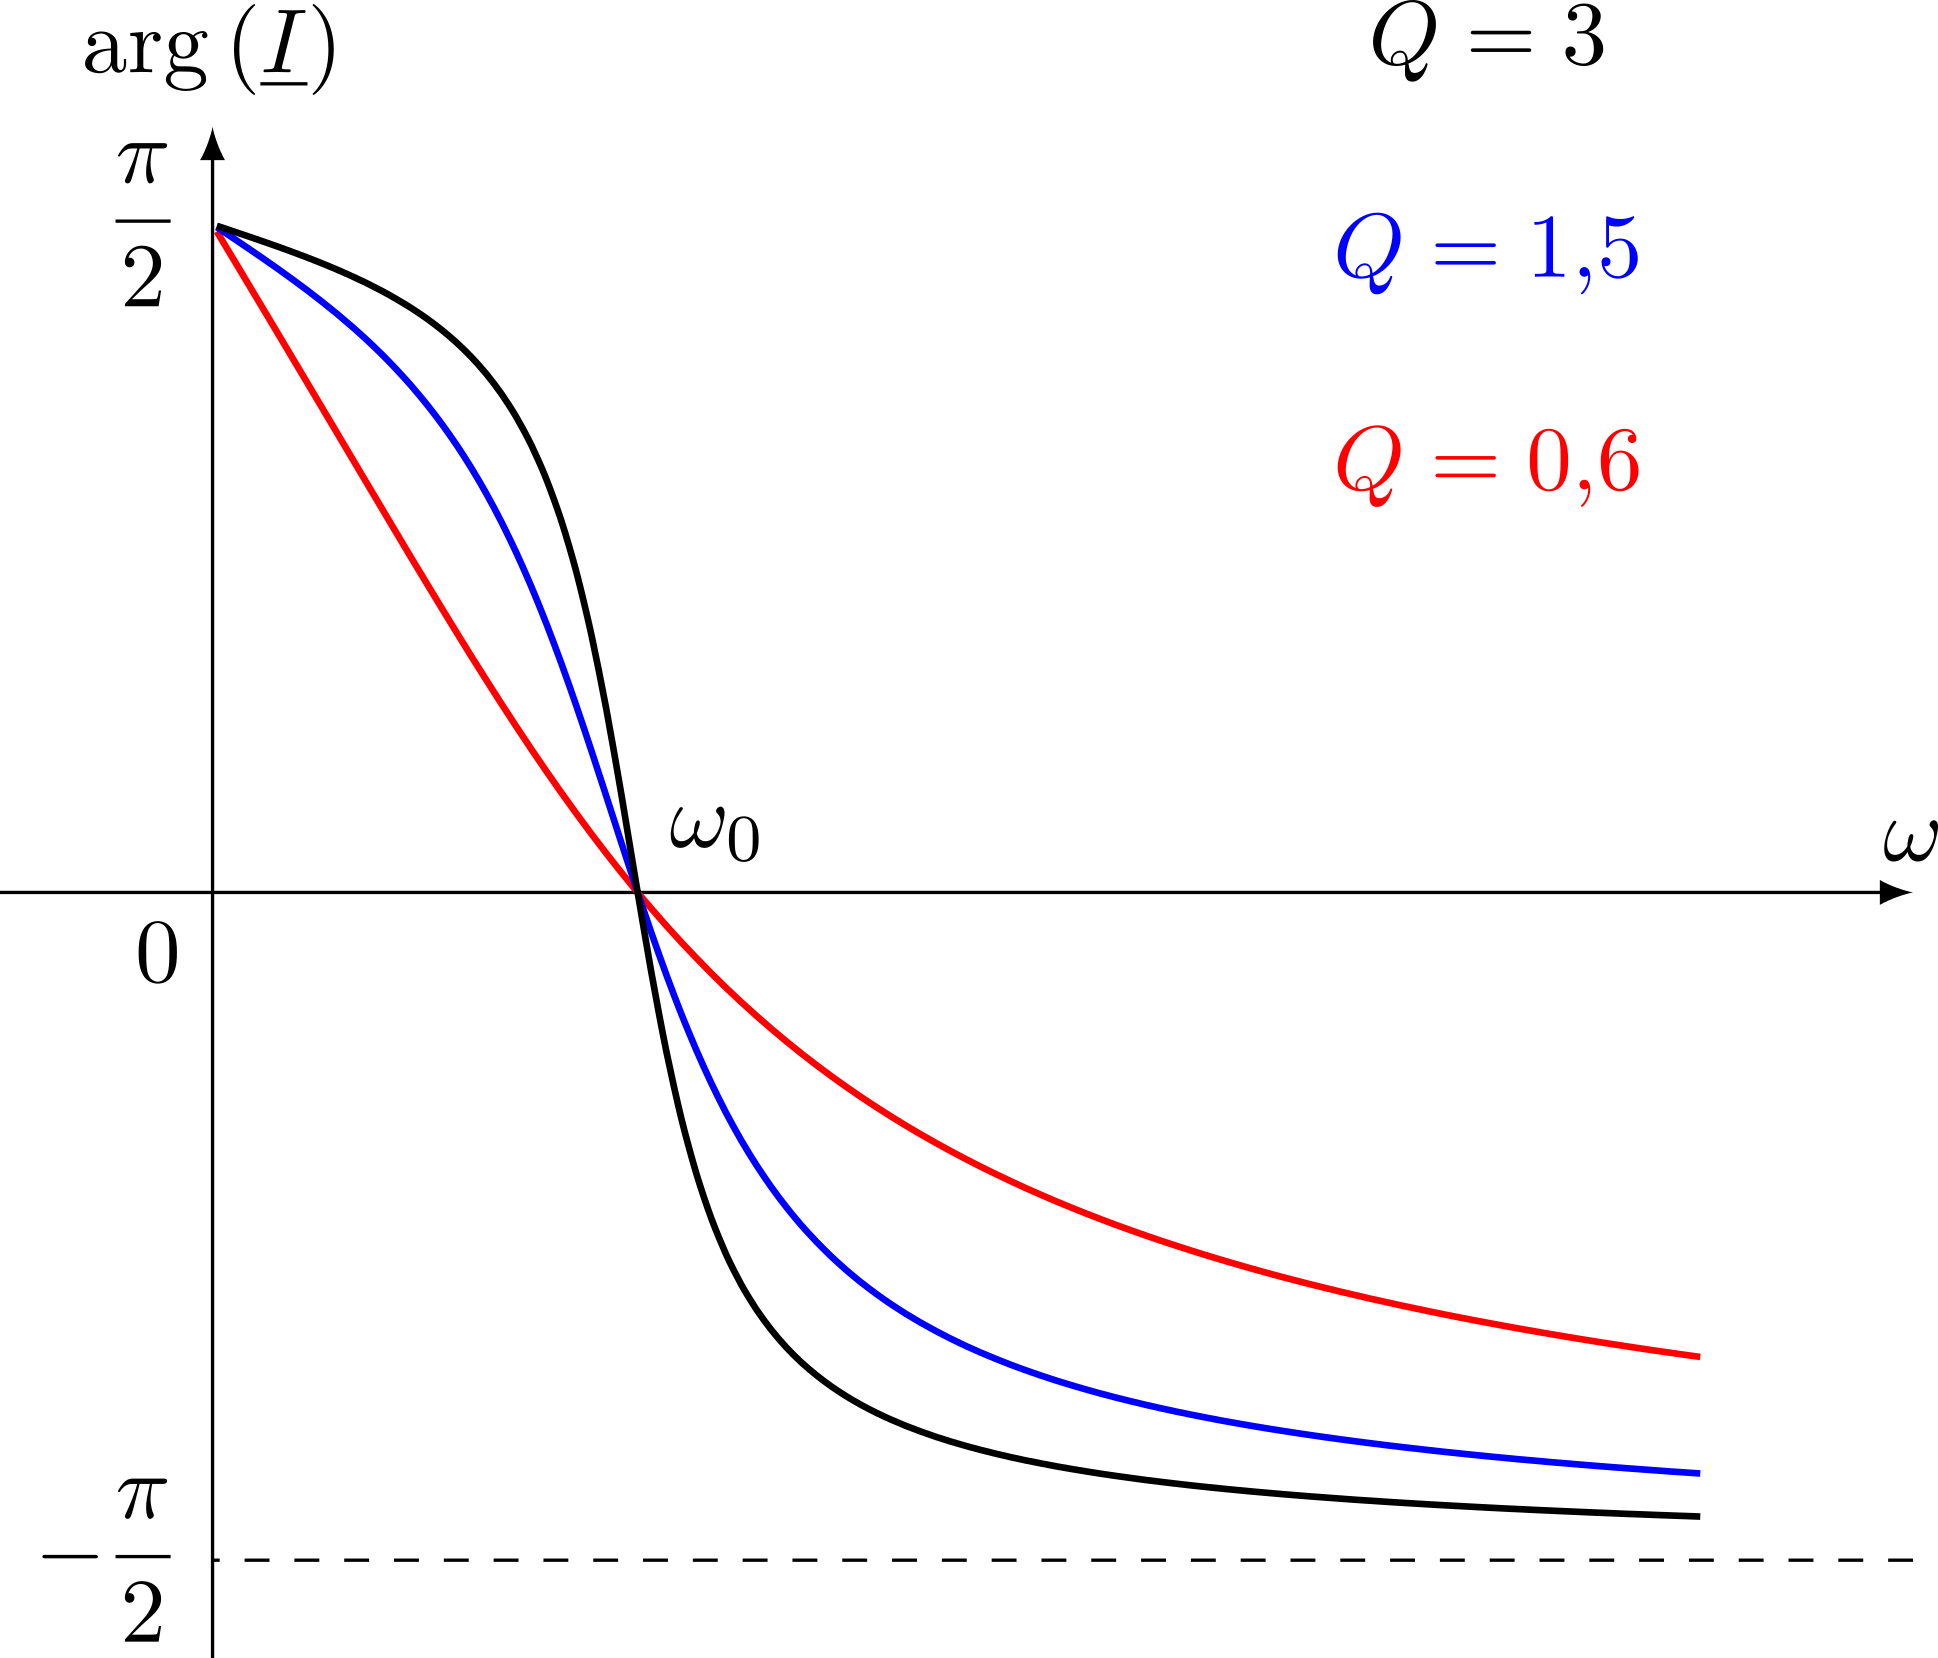
\includegraphics[width=.6\linewidth]{rlc_i-phase}
                              & 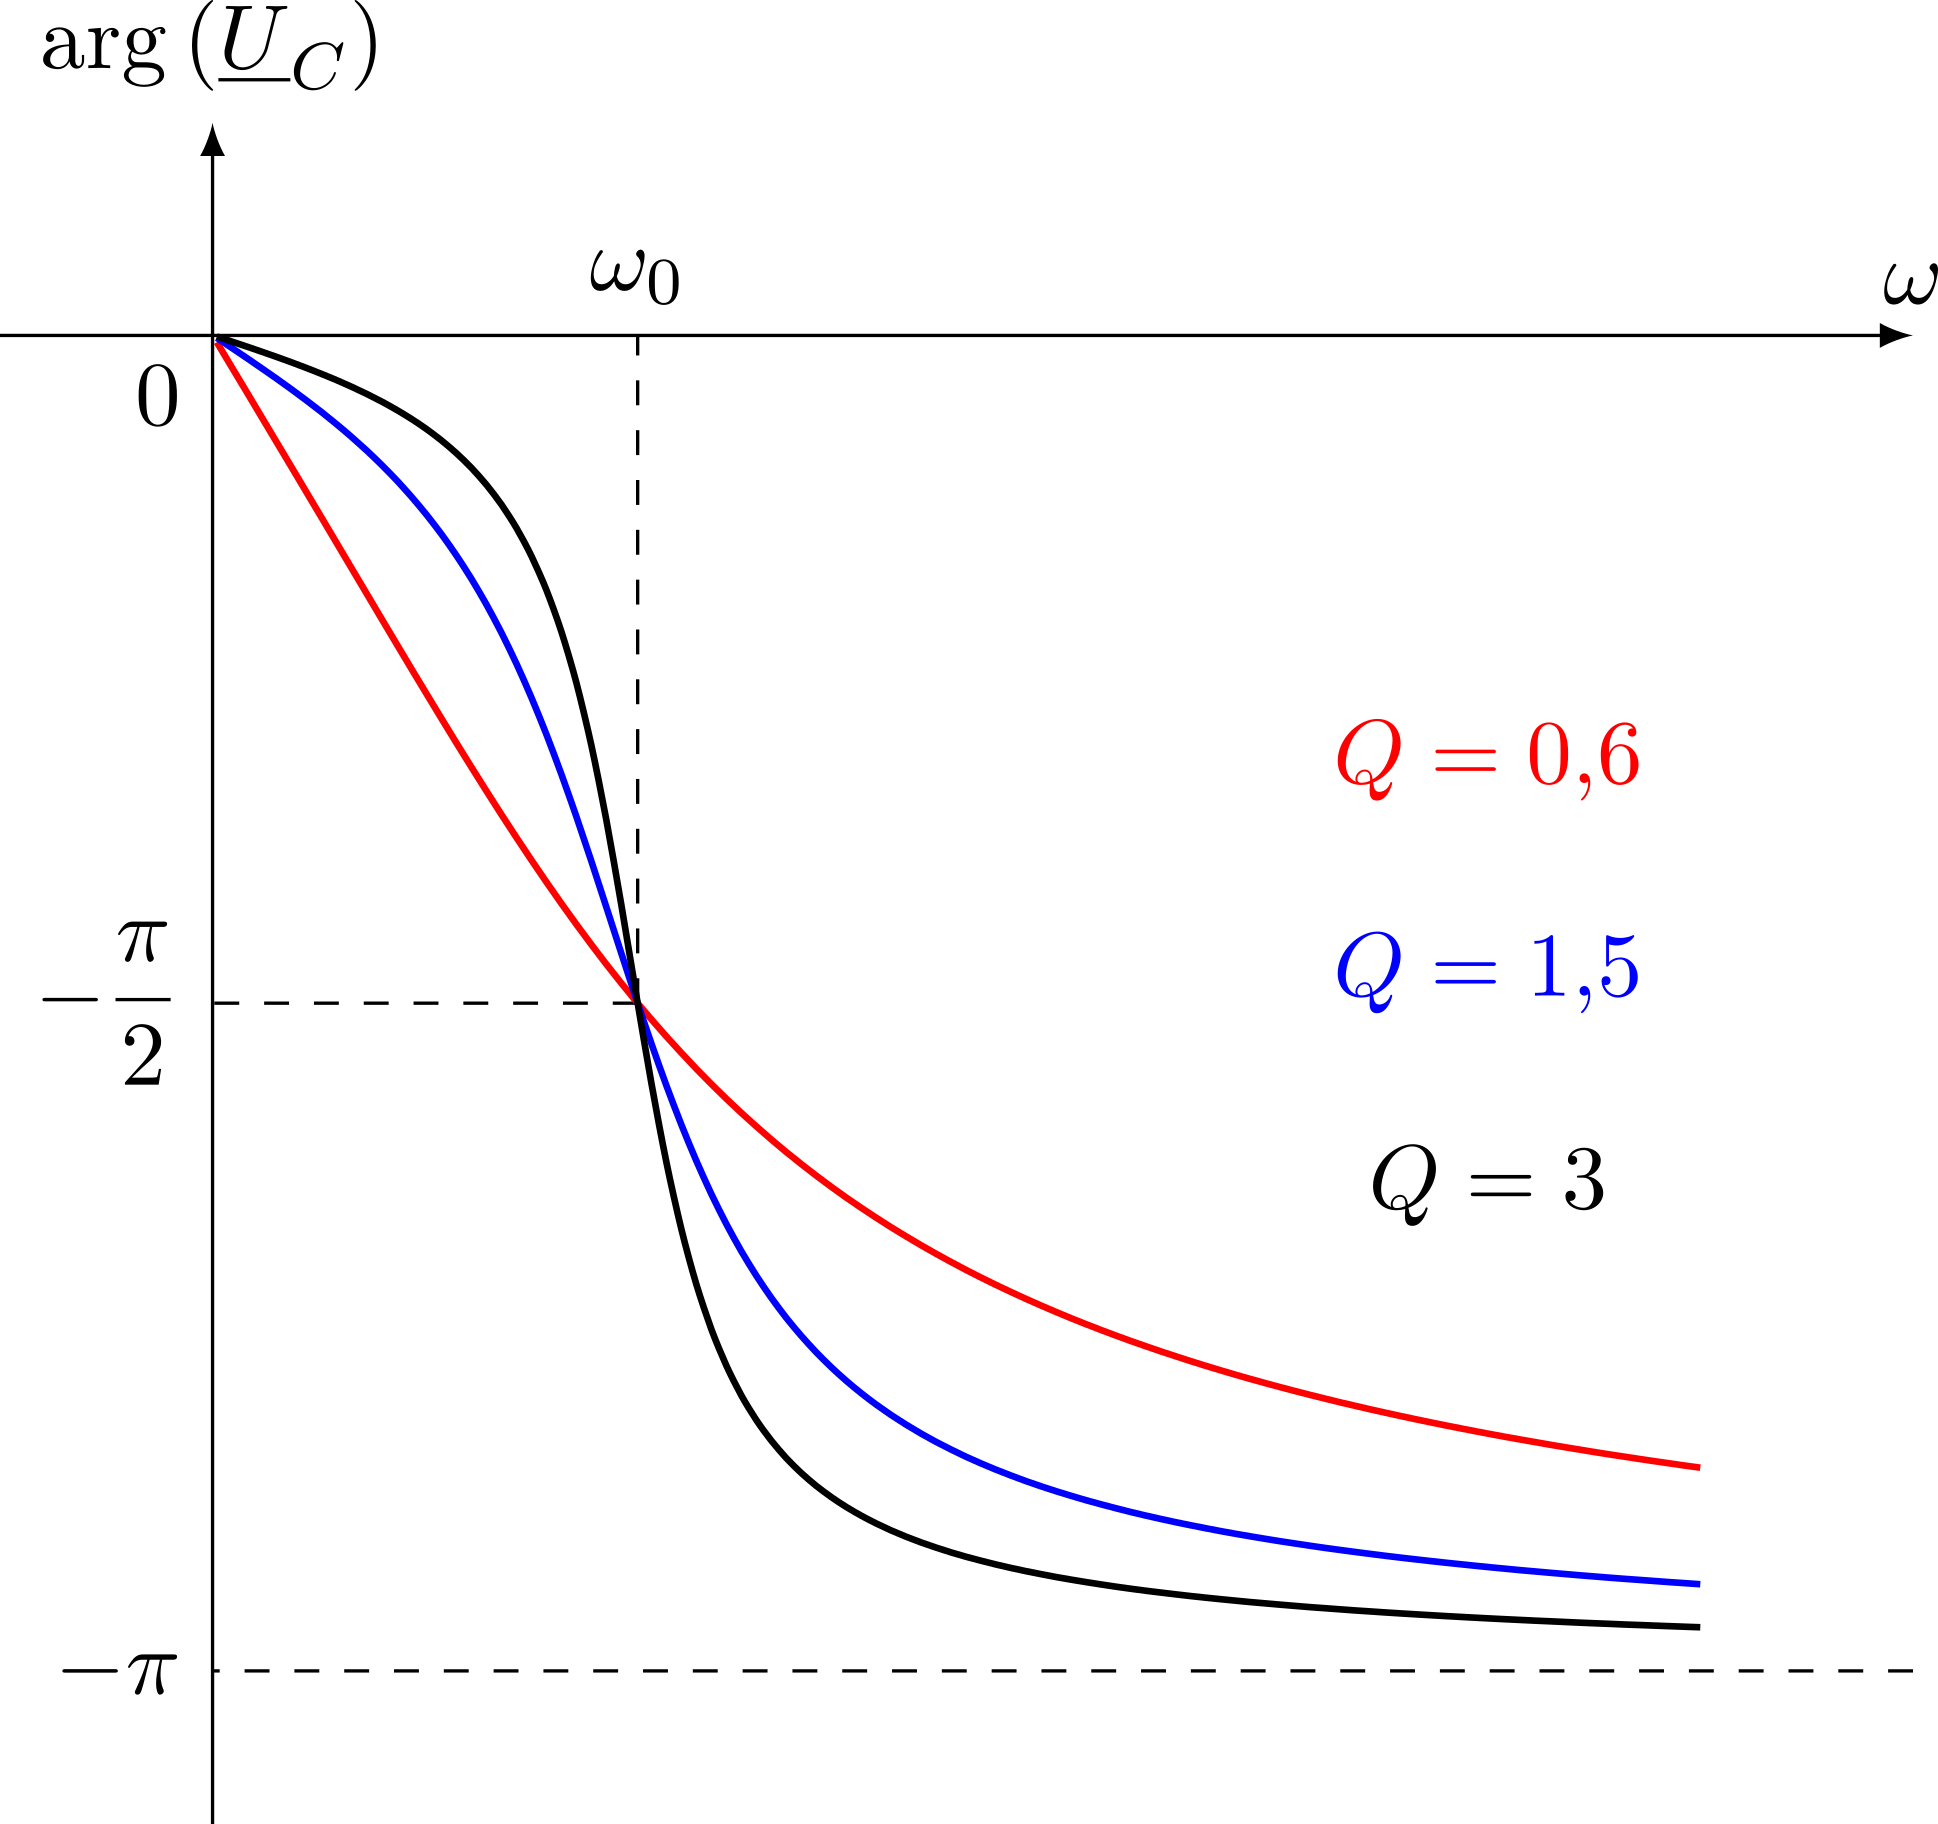
\includegraphics[width=.6\linewidth]{rlc_u-phase} 
\end{ror}

\end{document}
